% Part I — Foundations  |  ~6 slides  |  Madrid/seahorse  |  16:9
\documentclass[aspectratio=169,10pt]{beamer}
\usetheme{Madrid}\usecolortheme{seahorse}
\usepackage{tikz}
\usetikzlibrary{arrows.meta,shapes.geometric,positioning,calc,backgrounds}
\usepackage{pgfplots}\pgfplotsset{compat=1.17}
\usepackage{booktabs,amsmath,amssymb,xcolor}
\definecolor{myblue}{RGB}{0,50,130}
\definecolor{myred}{RGB}{153,0,0}
\definecolor{mygreen}{RGB}{0,100,50}
\definecolor{myorange}{RGB}{180,80,0}
\newcommand{\NHOP}{\mathrm{NHOP}}
\setbeamertemplate{navigation symbols}{}
\title[Part I: Foundations]{Part I — Foundations}
\subtitle{Class Imbalance: The Core Problem and Research Programme}
\author{Parsa Hajiannejad}\date{2026}

\begin{document}
\begin{frame}\titlepage\end{frame}

% ----- Slide 1 ---------------------------------------------------------------
\begin{frame}{SMOTE's Geometric Blind Spot}
\begin{columns}[T]
\column{0.44\textwidth}
\textbf{SMOTE} synthesises on a \textbf{line segment} between two minority points.
\vspace{6pt}
\begin{itemize}
  \item Covers only 1-D subspace between any pair — misses local 2-D neighbourhood
  \item Boundary-crossing risk: synthetic points land in majority territory
\end{itemize}
\vspace{6pt}
\textbf{Our claim:} replacing the segment with a \textbf{disk} (diameter = the two minority points) gives area-proportional 2-D coverage — while gravity weighting and angular biasing concentrate synthesis in safe, dense regions.

\column{0.54\textwidth}
\begin{center}
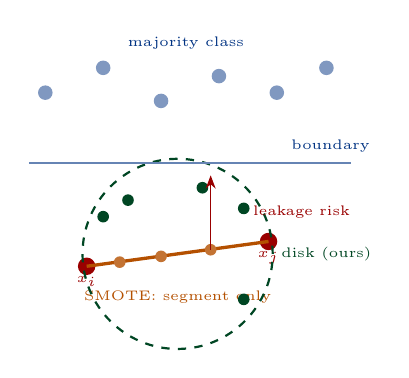
\begin{tikzpicture}[scale=1.05]
\foreach \x/\y in {0.2/3.0,0.9/3.3,1.6/2.9,2.3/3.2,3.0/3.0,3.6/3.3}
  {\fill[myblue!50] (\x,\y) circle (2.5pt);}
\node[font=\tiny,myblue] at (1.9,3.6) {majority class};
\fill[myred] (0.7,0.9) circle (3pt) node[below,font=\tiny]{$x_i$};
\fill[myred] (2.9,1.2) circle (3pt) node[below,font=\tiny]{$x_j$};
% SMOTE segment
\draw[myorange,very thick] (0.7,0.9) -- (2.9,1.2);
\node[font=\tiny,myorange,below] at (1.8,0.72) {SMOTE: segment only};
% Disk
\draw[mygreen!70!black,thick,dashed] (1.8,1.05) circle (1.15cm);
\node[font=\tiny,mygreen!70!black] at (3.6,1.05) {disk (ours)};
% SMOTE synth
\foreach \x/\y in {1.1/0.95,1.6/1.02,2.2/1.1}
  {\fill[myorange!80] (\x,\y) circle (2pt);}
% Disk synth
\foreach \x/\y in {1.2/1.7,2.1/1.85,2.6/0.5,0.9/1.5,2.6/1.6}
  {\fill[mygreen!70!black] (\x,\y) circle (2pt);}
% Decision boundary
\draw[myblue!60,thick] (-0.0,2.15) -- (3.9,2.15);
\node[font=\tiny,myblue] at (3.65,2.35) {boundary};
% Leakage arrow
\draw[-{Stealth},myred,thin] (2.2,1.1) -- (2.2,2.0);
\node[font=\tiny,myred] at (3.3,1.55) {leakage risk};
\end{tikzpicture}
\end{center}
\end{columns}
\end{frame}

% ----- Slide 2 ---------------------------------------------------------------
\begin{frame}{Four Gaps — Four Contributions}
\begin{columns}[T]
\column{0.50\textwidth}
Existing oversampling literature lacks:
\begin{center}
\begin{tabular}{@{}lll@{}}
\toprule
Gap & What is missing & This thesis \\
\midrule
G1 & Distributional fidelity measure & C1, C2 \\
G2 & Principled, geometry-aware seeds & C3 \\
G3 & 2-D (circular) synthesis & C4, C5 \\
G4 & Causal test: does IR itself degrade? & C6, C7 \\
\bottomrule
\end{tabular}
\end{center}
\vspace{4pt}
Leakage in existing benchmarks inflates AUC by \textbf{2–5\%} — reversing method rankings. Addressed by LeakageSafeCV (C6).

\column{0.48\textwidth}
\begin{tikzpicture}[
  wbox/.style={rectangle,rounded corners=4pt,draw,text width=4.6cm,
               align=left,font=\footnotesize,inner sep=6pt},
  arrow/.style={-{Stealth[length=5pt]},thick}]
\node[wbox,fill=myblue!12]   (c1) at (0,0)    {\textbf{C1–C2} NHOP + statistical theory\\$\NHOP_j = 1-\mathrm{TV}(P^j,Q^j)$};
\node[wbox,fill=mygreen!10]  (c3) at (0,-1.3) {\textbf{C3} Seed selection pipeline\\NHOP+AGTP−JSD composite criterion};
\node[wbox,fill=myorange!10] (c45) at (0,-2.6) {\textbf{C4–C5} GVM-CO / LRE-CO / LS-CO\\3 circular algorithms; +0.012–0.015 F1};
\node[wbox,fill=myred!10]    (c67) at (0,-3.9) {\textbf{C6–C7} Causal study + LeakageSafeCV\\1.4\% irreducible recovery gap (causal)};
\draw[arrow,myblue]   (c1.south)  -- (c3.north);
\draw[arrow,mygreen]  (c3.south)  -- (c45.north);
\draw[arrow,myorange] (c45.south) -- (c67.north);
\end{tikzpicture}
\end{columns}
\end{frame}

% ----- Slide 3 ---------------------------------------------------------------
\begin{frame}{Three Works Connected by One Metric}
\begin{center}
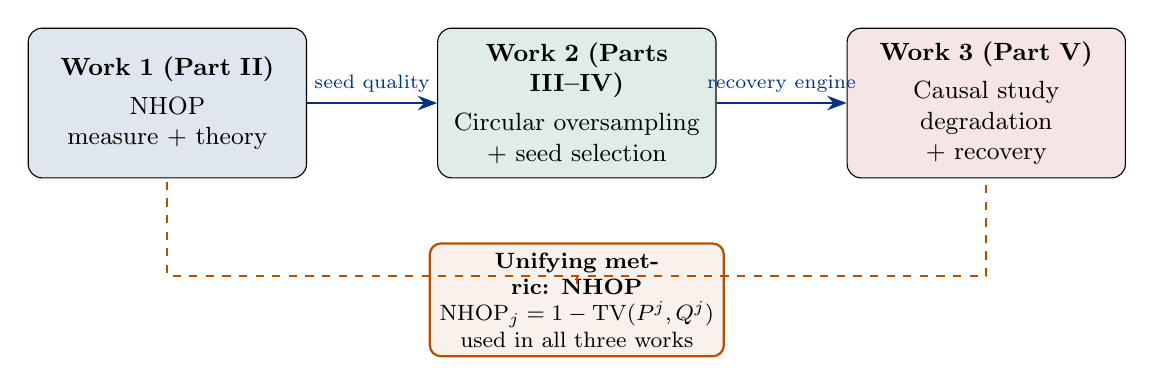
\begin{tikzpicture}[
  wbox/.style={rectangle,rounded corners=5pt,draw,fill=myblue!12,
               text width=3.3cm,align=center,font=\small,minimum height=1.9cm},
  arrow/.style={-{Stealth[length=7pt]},thick,myblue}]
\node[wbox] (w1) at (0,0)
  {\textbf{Work 1 (Part II)}\\\smallskip NHOP\\measure + theory};
\node[wbox,fill=mygreen!12] (w2) at (5.2,0)
  {\textbf{Work 2 (Parts III–IV)}\\\smallskip Circular oversampling\\+ seed selection};
\node[wbox,fill=myred!10] (w3) at (10.4,0)
  {\textbf{Work 3 (Part V)}\\\smallskip Causal study\\degradation + recovery};
\draw[arrow] (w1.east) -- node[above,font=\scriptsize]{seed quality} (w2.west);
\draw[arrow] (w2.east) -- node[above,font=\scriptsize]{recovery engine} (w3.west);
\node[draw=myorange,thick,rounded corners,fill=myorange!8,
      text width=3.5cm,align=center,font=\footnotesize] at (5.2,-2.5)
  {\textbf{Unifying metric: NHOP}\\
   $\NHOP_j=1-\mathrm{TV}(P^j,Q^j)$\\
   used in all three works};
\draw[myorange,dashed,thick] (0,-1.0) -- (0,-2.2) -- (10.4,-2.2) -- (10.4,-1.0);
\draw[myorange,dashed,thick] (5.2,-2.2) -- (5.2,-2.3);
\end{tikzpicture}
\end{center}
\vspace{4pt}
\begin{center}
\begin{tabular}{@{}lcccccc@{}}
\toprule
Part & I & II & III & IV & V & VI \\
Chapters & 1–3 & 4–5 & 6 & 7–11 & 12–16 & 17 \\
\bottomrule
\end{tabular}
\end{center}
\end{frame}

\end{document}
